\documentclass[1p]{elsarticle_modified}
%\bibliographystyle{elsarticle-num}

%\usepackage[colorlinks]{hyperref}
%\usepackage{abbrmath_seonhwa} %\Abb, \Ascr, \Acal ,\Abf, \Afrak
\usepackage{amsfonts}
\usepackage{amssymb}
\usepackage{amsmath}
\usepackage{amsthm}
\usepackage{scalefnt}
\usepackage{amsbsy}
\usepackage{kotex}
\usepackage{caption}
\usepackage{subfig}
\usepackage{color}
\usepackage{graphicx}
\usepackage{xcolor} %% white, black, red, green, blue, cyan, magenta, yellow
\usepackage{float}
\usepackage{setspace}
\usepackage{hyperref}

\usepackage{tikz}
\usetikzlibrary{arrows}

\usepackage{multirow}
\usepackage{array} % fixed length table
\usepackage{hhline}

%%%%%%%%%%%%%%%%%%%%%
\makeatletter
\renewcommand*\env@matrix[1][\arraystretch]{%
	\edef\arraystretch{#1}%
	\hskip -\arraycolsep
	\let\@ifnextchar\new@ifnextchar
	\array{*\c@MaxMatrixCols c}}
\makeatother %https://tex.stackexchange.com/questions/14071/how-can-i-increase-the-line-spacing-in-a-matrix
%%%%%%%%%%%%%%%

\usepackage[normalem]{ulem}

\newcommand{\msout}[1]{\ifmmode\text{\sout{\ensuremath{#1}}}\else\sout{#1}\fi}
%SOURCE: \msout is \stkout macro in https://tex.stackexchange.com/questions/20609/strikeout-in-math-mode

\newcommand{\cancel}[1]{
	\ifmmode
	{\color{red}\msout{#1}}
	\else
	{\color{red}\sout{#1}}
	\fi
}

\newcommand{\add}[1]{
	{\color{blue}\uwave{#1}}
}

\newcommand{\replace}[2]{
	\ifmmode
	{\color{red}\msout{#1}}{\color{blue}\uwave{#2}}
	\else
	{\color{red}\sout{#1}}{\color{blue}\uwave{#2}}
	\fi
}

\newcommand{\Sol}{\mathcal{S}} %segment
\newcommand{\D}{D} %diagram
\newcommand{\A}{\mathcal{A}} %arc


%%%%%%%%%%%%%%%%%%%%%%%%%%%%%5 test

\def\sl{\operatorname{\textup{SL}}(2,\Cbb)}
\def\psl{\operatorname{\textup{PSL}}(2,\Cbb)}
\def\quan{\mkern 1mu \triangleright \mkern 1mu}

\theoremstyle{definition}
\newtheorem{thm}{Theorem}[section]
\newtheorem{prop}[thm]{Proposition}
\newtheorem{lem}[thm]{Lemma}
\newtheorem{ques}[thm]{Question}
\newtheorem{cor}[thm]{Corollary}
\newtheorem{defn}[thm]{Definition}
\newtheorem{exam}[thm]{Example}
\newtheorem{rmk}[thm]{Remark}
\newtheorem{alg}[thm]{Algorithm}

\newcommand{\I}{\sqrt{-1}}
\begin{document}

%\begin{frontmatter}
%
%\title{Boundary parabolic representations of knots up to 8 crossings}
%
%%% Group authors per affiliation:
%\author{Yunhi Cho} 
%\address{Department of Mathematics, University of Seoul, Seoul, Korea}
%\ead{yhcho@uos.ac.kr}
%
%
%\author{Seonhwa Kim} %\fnref{s_kim}}
%\address{Center for Geometry and Physics, Institute for Basic Science, Pohang, 37673, Korea}
%\ead{ryeona17@ibs.re.kr}
%
%\author{Hyuk Kim}
%\address{Department of Mathematical Sciences, Seoul National University, Seoul 08826, Korea}
%\ead{hyukkim@snu.ac.kr}
%
%\author{Seokbeom Yoon}
%\address{Department of Mathematical Sciences, Seoul National University, Seoul, 08826,  Korea}
%\ead{sbyoon15@snu.ac.kr}
%
%\begin{abstract}
%We find all boundary parabolic representation of knots up to 8 crossings.
%
%\end{abstract}
%\begin{keyword}
%    \MSC[2010] 57M25 
%\end{keyword}
%
%\end{frontmatter}

%\linenumbers
%\tableofcontents
%
\newcommand\colored[1]{\textcolor{white}{\rule[-0.35ex]{0.8em}{1.4ex}}\kern-0.8em\color{red} #1}%
%\newcommand\colored[1]{\textcolor{white}{ #1}\kern-2.17ex	\textcolor{white}{ #1}\kern-1.81ex	\textcolor{white}{ #1}\kern-2.15ex\color{red}#1	}

{\Large $\underline{12a_{0668}~(K12a_{0668})}$}

\setlength{\tabcolsep}{10pt}
\renewcommand{\arraystretch}{1.6}
\vspace{1cm}\begin{tabular}{m{100pt}>{\centering\arraybackslash}m{274pt}}
\multirow{5}{120pt}{
	\centering
	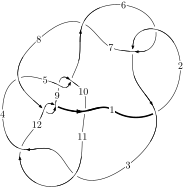
\includegraphics[width=112pt]{../../../GIT/diagram.site/Diagrams/png/1469_12a_0668.png}\\
\ \ \ A knot diagram\footnotemark}&
\allowdisplaybreaks
\textbf{Linearized knot diagam} \\
\cline{2-2}
 &
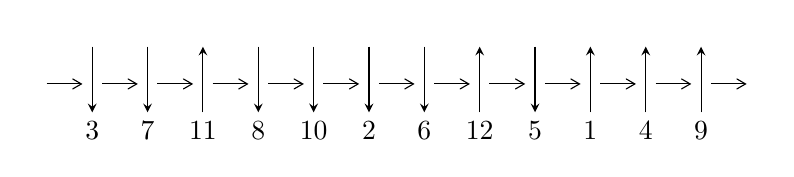
\begin{tikzpicture}[x=20pt, y=17pt]
	% nodes
	\node (C0) at (0, 0) {};
	\node (C1) at (1, 0) {};
	\node (C1U) at (1, +1) {};
	\node (C1D) at (1, -1) {3};

	\node (C2) at (2, 0) {};
	\node (C2U) at (2, +1) {};
	\node (C2D) at (2, -1) {7};

	\node (C3) at (3, 0) {};
	\node (C3U) at (3, +1) {};
	\node (C3D) at (3, -1) {11};

	\node (C4) at (4, 0) {};
	\node (C4U) at (4, +1) {};
	\node (C4D) at (4, -1) {8};

	\node (C5) at (5, 0) {};
	\node (C5U) at (5, +1) {};
	\node (C5D) at (5, -1) {10};

	\node (C6) at (6, 0) {};
	\node (C6U) at (6, +1) {};
	\node (C6D) at (6, -1) {2};

	\node (C7) at (7, 0) {};
	\node (C7U) at (7, +1) {};
	\node (C7D) at (7, -1) {6};

	\node (C8) at (8, 0) {};
	\node (C8U) at (8, +1) {};
	\node (C8D) at (8, -1) {12};

	\node (C9) at (9, 0) {};
	\node (C9U) at (9, +1) {};
	\node (C9D) at (9, -1) {5};

	\node (C10) at (10, 0) {};
	\node (C10U) at (10, +1) {};
	\node (C10D) at (10, -1) {1};

	\node (C11) at (11, 0) {};
	\node (C11U) at (11, +1) {};
	\node (C11D) at (11, -1) {4};

	\node (C12) at (12, 0) {};
	\node (C12U) at (12, +1) {};
	\node (C12D) at (12, -1) {9};
	\node (C13) at (13, 0) {};

	% arrows
	\draw[->,>={angle 60}]
	(C0) edge (C1) (C1) edge (C2) (C2) edge (C3) (C3) edge (C4) (C4) edge (C5) (C5) edge (C6) (C6) edge (C7) (C7) edge (C8) (C8) edge (C9) (C9) edge (C10) (C10) edge (C11) (C11) edge (C12) (C12) edge (C13) ;	\draw[->,>=stealth]
	(C1U) edge (C1D) (C2U) edge (C2D) (C3D) edge (C3U) (C4U) edge (C4D) (C5U) edge (C5D) (C6U) edge (C6D) (C7U) edge (C7D) (C8D) edge (C8U) (C9U) edge (C9D) (C10D) edge (C10U) (C11D) edge (C11U) (C12D) edge (C12U) ;
	\end{tikzpicture} \\
\hhline{~~} \\& 
\textbf{Solving Sequence} \\ \cline{2-2} 
 &
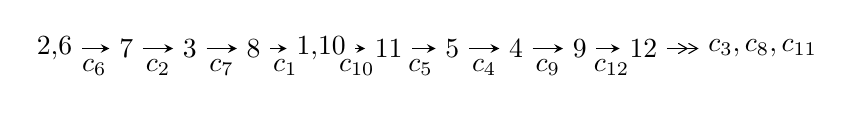
\begin{tikzpicture}[x=23pt, y=7pt]
	% node
	\node (A0) at (-1/8, 0) {2,6};
	\node (A1) at (1, 0) {7};
	\node (A2) at (2, 0) {3};
	\node (A3) at (3, 0) {8};
	\node (A4) at (65/16, 0) {1,10};
	\node (A5) at (41/8, 0) {11};
	\node (A6) at (49/8, 0) {5};
	\node (A7) at (57/8, 0) {4};
	\node (A8) at (65/8, 0) {9};
	\node (A9) at (73/8, 0) {12};
	\node (C1) at (1/2, -1) {$c_{6}$};
	\node (C2) at (3/2, -1) {$c_{2}$};
	\node (C3) at (5/2, -1) {$c_{7}$};
	\node (C4) at (7/2, -1) {$c_{1}$};
	\node (C5) at (37/8, -1) {$c_{10}$};
	\node (C6) at (45/8, -1) {$c_{5}$};
	\node (C7) at (53/8, -1) {$c_{4}$};
	\node (C8) at (61/8, -1) {$c_{9}$};
	\node (C9) at (69/8, -1) {$c_{12}$};
	\node (A10) at (11, 0) {$c_{3},c_{8},c_{11}$};

	% edge
	\draw[->,>=stealth]	
	(A0) edge (A1) (A1) edge (A2) (A2) edge (A3) (A3) edge (A4) (A4) edge (A5) (A5) edge (A6) (A6) edge (A7) (A7) edge (A8) (A8) edge (A9) ;
	\draw[->>,>={angle 60}]	
	(A9) edge (A10);
\end{tikzpicture} \\ 

\end{tabular} \\

\footnotetext{
The image of knot diagram is generated by the software ``\textbf{Draw programme}" developed by Andrew Bartholomew(\url{http://www.layer8.co.uk/maths/draw/index.htm\#Running-draw}), where we modified some parts for our purpose(\url{https://github.com/CATsTAILs/LinksPainter}).
}\phantom \\ \newline 
\centering \textbf{Ideals for irreducible components\footnotemark of $X_{\text{par}}$} 
 
\begin{align*}
I^u_{1}&=\langle 
-192 u^{76}-372 u^{75}+\cdots+2304 b+776,\;-4833 u^{76}-10270 u^{75}+\cdots+52992 a+144168,\\
\phantom{I^u_{1}}&\phantom{= \langle  }u^{77}+4 u^{76}+\cdots-32 u+46\rangle \\
I^u_{2}&=\langle 
b+1,\;- u^3-8 u^2+10 a-2 u+14,\;u^4-2 u^2+2\rangle \\
I^u_{3}&=\langle 
-6 a^2 u^2+7 a^2 u- u^2 a+2 a^2-2 a u+2 u^2+19 b+13 a+4 u+12,\;a^3+2 a^2 u-2 a^2+a u+u^2+a- u-2,\\
\phantom{I^u_{3}}&\phantom{= \langle  }u^3- u^2+1\rangle \\
I^u_{4}&=\langle 
- b^2 u^2 a+b^2 a u+b^3+u^2 b+u^2 a- b u- a u- u^2- b+u-1,\;u^3- u^2+1\rangle \\
\\
I^v_{1}&=\langle 
a,\;b^3- b+1,\;v-1\rangle \\
I^v_{2}&=\langle 
a,\;b-1,\;v-1\rangle \\
\end{align*}
\raggedright * 5 irreducible components of $\dim_{\mathbb{C}}=0$, with total 94 representations.\\
\raggedright * 1 irreducible components of $\dim_{\mathbb{C}}=1$ \\
\footnotetext{All coefficients of polynomials are rational numbers. But the coefficients are sometimes approximated in decimal forms when there is not enough margin.}
\newpage
\renewcommand{\arraystretch}{1}
\centering \section*{I. $I^u_{1}= \langle -192 u^{76}-372 u^{75}+\cdots+2304 b+776,\;-4833 u^{76}-10270 u^{75}+\cdots+52992 a+144168,\;u^{77}+4 u^{76}+\cdots-32 u+46 \rangle$}
\flushleft \textbf{(i) Arc colorings}\\
\begin{tabular}{m{7pt} m{180pt} m{7pt} m{180pt} }
\flushright $a_{2}=$&$\begin{pmatrix}0\\u\end{pmatrix}$ \\
\flushright $a_{6}=$&$\begin{pmatrix}1\\0\end{pmatrix}$ \\
\flushright $a_{7}=$&$\begin{pmatrix}1\\u^2\end{pmatrix}$ \\
\flushright $a_{3}=$&$\begin{pmatrix}- u\\- u^3+u\end{pmatrix}$ \\
\flushright $a_{8}=$&$\begin{pmatrix}- u^2+1\\u^2\end{pmatrix}$ \\
\flushright $a_{1}=$&$\begin{pmatrix}u^3\\u^5- u^3+u\end{pmatrix}$ \\
\flushright $a_{10}=$&$\begin{pmatrix}0.0912024 u^{76}+0.193803 u^{75}+\cdots+0.310198 u-2.72056\\0.0833333 u^{76}+0.161458 u^{75}+\cdots+3.90538 u-0.336806\end{pmatrix}$ \\
\flushright $a_{11}=$&$\begin{pmatrix}-0.256454 u^{76}-0.885624 u^{75}+\cdots+7.09666 u-12.3039\\0.375000 u^{76}+0.894531 u^{75}+\cdots+9.90799 u+2.05903\end{pmatrix}$ \\
\flushright $a_{5}=$&$\begin{pmatrix}-0.0515172 u^{76}-0.0498188 u^{75}+\cdots-4.84681 u+4.73970\\-0.00520833 u^{76}-0.0716146 u^{75}+\cdots+3.14583 u-1.83073\end{pmatrix}$ \\
\flushright $a_{4}=$&$\begin{pmatrix}0.0448370 u^{76}+0.127264 u^{75}+\cdots+1.43965 u+2.90897\\0.0234375 u^{76}+0.145833 u^{75}+\cdots-5.97917 u+3.02083\end{pmatrix}$ \\
\flushright $a_{9}=$&$\begin{pmatrix}-0.694407 u^{76}-1.99580 u^{75}+\cdots+9.07051 u-19.4422\\0.222222 u^{76}+0.331597 u^{75}+\cdots+20.5932 u-5.01620\end{pmatrix}$ \\
\flushright $a_{12}=$&$\begin{pmatrix}0.672781 u^{76}+1.91826 u^{75}+\cdots-11.6092 u+14.8391\\-0.184028 u^{76}-0.301215 u^{75}+\cdots-14.0162 u+3.60880\end{pmatrix}$\\&\end{tabular}
\flushleft \textbf{(ii) Obstruction class $= -1$}\\~\\
\flushleft \textbf{(iii) Cusp Shapes $= -\frac{677}{576} u^{76}-\frac{233}{54} u^{75}+\cdots+\frac{6815}{72} u-\frac{5585}{108}$}\\~\\
\newpage\renewcommand{\arraystretch}{1}
\flushleft \textbf{(iv) u-Polynomials at the component}\newline \\
\begin{tabular}{m{50pt}|m{274pt}}
Crossings & \hspace{64pt}u-Polynomials at each crossing \\
\hline $$\begin{aligned}c_{1},c_{7}\end{aligned}$$&$\begin{aligned}
&u^{77}+24 u^{76}+\cdots+23104 u+2116
\end{aligned}$\\
\hline $$\begin{aligned}c_{2},c_{6}\end{aligned}$$&$\begin{aligned}
&u^{77}+4 u^{76}+\cdots-32 u+46
\end{aligned}$\\
\hline $$\begin{aligned}c_{3},c_{11}\end{aligned}$$&$\begin{aligned}
&27(27 u^{77}-54 u^{76}+\cdots-329 u-49)
\end{aligned}$\\
\hline $$\begin{aligned}c_{4}\end{aligned}$$&$\begin{aligned}
&64(64 u^{77}-64 u^{76}+\cdots-7193097 u-7328259)
\end{aligned}$\\
\hline $$\begin{aligned}c_{5},c_{9}\end{aligned}$$&$\begin{aligned}
&27(27 u^{77}+54 u^{76}+\cdots+259 u-49)
\end{aligned}$\\
\hline $$\begin{aligned}c_{8},c_{12}\end{aligned}$$&$\begin{aligned}
&u^{77}+8 u^{76}+\cdots+288144 u+24982
\end{aligned}$\\
\hline $$\begin{aligned}c_{10}\end{aligned}$$&$\begin{aligned}
&64(64 u^{77}+192 u^{76}+\cdots+2.57763\times10^{7} u-4.07362\times10^{7})
\end{aligned}$\\
\hline
\end{tabular}\\~\\
\newpage\renewcommand{\arraystretch}{1}
\flushleft \textbf{(v) Riley Polynomials at the component}\newline \\
\begin{tabular}{m{50pt}|m{274pt}}
Crossings & \hspace{64pt}Riley Polynomials at each crossing \\
\hline $$\begin{aligned}c_{1},c_{7}\end{aligned}$$&$\begin{aligned}
&y^{77}+60 y^{76}+\cdots+169876672 y-4477456
\end{aligned}$\\
\hline $$\begin{aligned}c_{2},c_{6}\end{aligned}$$&$\begin{aligned}
&y^{77}-24 y^{76}+\cdots+23104 y-2116
\end{aligned}$\\
\hline $$\begin{aligned}c_{3},c_{11}\end{aligned}$$&$\begin{aligned}
&729(729 y^{77}-49572 y^{76}+\cdots+20923 y-2401)
\end{aligned}$\\
\hline $$\begin{aligned}c_{4}\end{aligned}$$&$\begin{aligned}
&4096\\
&\cdot(4096 y^{77}+192512 y^{76}+\cdots-759954294636435 y-53703379971081)
\end{aligned}$\\
\hline $$\begin{aligned}c_{5},c_{9}\end{aligned}$$&$\begin{aligned}
&729(729 y^{77}-26244 y^{76}+\cdots+150283 y-2401)
\end{aligned}$\\
\hline $$\begin{aligned}c_{8},c_{12}\end{aligned}$$&$\begin{aligned}
&y^{77}-44 y^{76}+\cdots+27288625256 y-624100324
\end{aligned}$\\
\hline $$\begin{aligned}c_{10}\end{aligned}$$&$\begin{aligned}
&4096(4096 y^{77}-208896 y^{76}+\cdots+3.66690\times10^{16} y-1.65944\times10^{15})
\end{aligned}$\\
\hline
\end{tabular}\\~\\
\newpage\flushleft \textbf{(vi) Complex Volumes and Cusp Shapes}
$$\begin{array}{c|c|c}  
\text{Solutions to }I^u_{1}& \I (\text{vol} + \sqrt{-1}CS) & \text{Cusp shape}\\
 \hline 
\begin{aligned}
u &= -0.945096 + 0.389047 I \\
a &= -0.050623 - 1.070080 I \\
b &= -1.137580 - 0.286797 I\end{aligned}
 & -2.25647 - 1.16651 I & \phantom{-0.000000 } 0 \\ \hline\begin{aligned}
u &= -0.945096 - 0.389047 I \\
a &= -0.050623 + 1.070080 I \\
b &= -1.137580 + 0.286797 I\end{aligned}
 & -2.25647 + 1.16651 I & \phantom{-0.000000 } 0 \\ \hline\begin{aligned}
u &= \phantom{-}1.013910 + 0.200035 I \\
a &= -1.38511 + 0.76890 I \\
b &= -1.264600 - 0.574600 I\end{aligned}
 & -3.31072 - 7.02161 I & \phantom{-0.000000 -}0. + 7.58050 I \\ \hline\begin{aligned}
u &= \phantom{-}1.013910 - 0.200035 I \\
a &= -1.38511 - 0.76890 I \\
b &= -1.264600 + 0.574600 I\end{aligned}
 & -3.31072 + 7.02161 I & \phantom{-0.000000 } 0. - 7.58050 I \\ \hline\begin{aligned}
u &= \phantom{-}0.990472 + 0.339163 I \\
a &= \phantom{-}0.261413 + 0.088872 I \\
b &= -0.074059 + 0.966853 I\end{aligned}
 & \phantom{-}4.92520 - 6.64796 I & \phantom{-0.000000 } 0 \\ \hline\begin{aligned}
u &= \phantom{-}0.990472 - 0.339163 I \\
a &= \phantom{-}0.261413 - 0.088872 I \\
b &= -0.074059 - 0.966853 I\end{aligned}
 & \phantom{-}4.92520 + 6.64796 I & \phantom{-0.000000 } 0 \\ \hline\begin{aligned}
u &= \phantom{-}1.038030 + 0.149643 I \\
a &= \phantom{-}1.43369 - 0.68788 I \\
b &= \phantom{-}1.211790 + 0.261921 I\end{aligned}
 & -5.95131 - 2.26654 I & \phantom{-0.000000 } 0 \\ \hline\begin{aligned}
u &= \phantom{-}1.038030 - 0.149643 I \\
a &= \phantom{-}1.43369 + 0.68788 I \\
b &= \phantom{-}1.211790 - 0.261921 I\end{aligned}
 & -5.95131 + 2.26654 I & \phantom{-0.000000 } 0 \\ \hline\begin{aligned}
u &= -0.731824 + 0.784777 I \\
a &= \phantom{-}0.776824 + 0.762762 I \\
b &= -1.101830 - 0.505985 I\end{aligned}
 & \phantom{-}0.30848 - 1.84699 I & \phantom{-0.000000 } 0 \\ \hline\begin{aligned}
u &= -0.731824 - 0.784777 I \\
a &= \phantom{-}0.776824 - 0.762762 I \\
b &= -1.101830 + 0.505985 I\end{aligned}
 & \phantom{-}0.30848 + 1.84699 I & \phantom{-0.000000 } 0\\
 \hline 
 \end{array}$$\newpage$$\begin{array}{c|c|c}  
\text{Solutions to }I^u_{1}& \I (\text{vol} + \sqrt{-1}CS) & \text{Cusp shape}\\
 \hline 
\begin{aligned}
u &= \phantom{-}0.853104 + 0.340329 I \\
a &= \phantom{-}0.213746 + 0.784050 I \\
b &= -0.255176 - 0.454138 I\end{aligned}
 & \phantom{-}0.14615 - 3.23036 I & -1.33855 + 8.12824 I \\ \hline\begin{aligned}
u &= \phantom{-}0.853104 - 0.340329 I \\
a &= \phantom{-}0.213746 - 0.784050 I \\
b &= -0.255176 + 0.454138 I\end{aligned}
 & \phantom{-}0.14615 + 3.23036 I & -1.33855 - 8.12824 I \\ \hline\begin{aligned}
u &= \phantom{-}0.914885\phantom{ +0.000000I} \\
a &= -3.07046\phantom{ +0.000000I} \\
b &= -0.837226\phantom{ +0.000000I}\end{aligned}
 & -0.405134\phantom{ +0.000000I} & -11.6500\phantom{ +0.000000I} \\ \hline\begin{aligned}
u &= -0.796108 + 0.747982 I \\
a &= -0.10708 - 1.46416 I \\
b &= \phantom{-}0.752389 + 0.337777 I\end{aligned}
 & \phantom{-}4.41618 + 1.21466 I & \phantom{-0.000000 } 0 \\ \hline\begin{aligned}
u &= -0.796108 - 0.747982 I \\
a &= -0.10708 + 1.46416 I \\
b &= \phantom{-}0.752389 - 0.337777 I\end{aligned}
 & \phantom{-}4.41618 - 1.21466 I & \phantom{-0.000000 } 0 \\ \hline\begin{aligned}
u &= -1.090320 + 0.129993 I \\
a &= -1.262460 + 0.002905 I \\
b &= -0.404038 + 0.480402 I\end{aligned}
 & \phantom{-}3.57275 - 0.38450 I & \phantom{-0.000000 } 0 \\ \hline\begin{aligned}
u &= -1.090320 - 0.129993 I \\
a &= -1.262460 - 0.002905 I \\
b &= -0.404038 - 0.480402 I\end{aligned}
 & \phantom{-}3.57275 + 0.38450 I & \phantom{-0.000000 } 0 \\ \hline\begin{aligned}
u &= -0.745520 + 0.814582 I \\
a &= -1.16110 - 1.01142 I \\
b &= \phantom{-}1.19077 + 0.83255 I\end{aligned}
 & \phantom{-}3.35457 - 6.24610 I & \phantom{-0.000000 } 0 \\ \hline\begin{aligned}
u &= -0.745520 - 0.814582 I \\
a &= -1.16110 + 1.01142 I \\
b &= \phantom{-}1.19077 - 0.83255 I\end{aligned}
 & \phantom{-}3.35457 + 6.24610 I & \phantom{-0.000000 } 0 \\ \hline\begin{aligned}
u &= \phantom{-}0.143068 + 0.884102 I \\
a &= \phantom{-}0.168538 + 0.574471 I \\
b &= -0.837315 - 0.407607 I\end{aligned}
 & \phantom{-}1.74848 - 1.75393 I & \phantom{-}4.13656 + 4.20451 I\\
 \hline 
 \end{array}$$\newpage$$\begin{array}{c|c|c}  
\text{Solutions to }I^u_{1}& \I (\text{vol} + \sqrt{-1}CS) & \text{Cusp shape}\\
 \hline 
\begin{aligned}
u &= \phantom{-}0.143068 - 0.884102 I \\
a &= \phantom{-}0.168538 - 0.574471 I \\
b &= -0.837315 + 0.407607 I\end{aligned}
 & \phantom{-}1.74848 + 1.75393 I & \phantom{-}4.13656 - 4.20451 I \\ \hline\begin{aligned}
u &= \phantom{-}0.672918 + 0.883872 I \\
a &= -0.114733 + 0.792856 I \\
b &= \phantom{-}0.786004 - 0.691152 I\end{aligned}
 & \phantom{-}10.55870 + 0.08501 I & \phantom{-0.000000 } 0 \\ \hline\begin{aligned}
u &= \phantom{-}0.672918 - 0.883872 I \\
a &= -0.114733 - 0.792856 I \\
b &= \phantom{-}0.786004 + 0.691152 I\end{aligned}
 & \phantom{-}10.55870 - 0.08501 I & \phantom{-0.000000 } 0 \\ \hline\begin{aligned}
u &= \phantom{-}0.833547 + 0.780072 I \\
a &= -1.32633 - 0.56782 I \\
b &= \phantom{-}0.720819 + 0.274380 I\end{aligned}
 & \phantom{-}4.51444 - 3.95451 I & \phantom{-0.000000 } 0 \\ \hline\begin{aligned}
u &= \phantom{-}0.833547 - 0.780072 I \\
a &= -1.32633 + 0.56782 I \\
b &= \phantom{-}0.720819 - 0.274380 I\end{aligned}
 & \phantom{-}4.51444 + 3.95451 I & \phantom{-0.000000 } 0 \\ \hline\begin{aligned}
u &= -1.033180 + 0.514901 I \\
a &= \phantom{-}0.384364 + 1.026620 I \\
b &= \phantom{-}1.154440 + 0.045045 I\end{aligned}
 & -3.87527 + 4.08507 I & \phantom{-0.000000 } 0 \\ \hline\begin{aligned}
u &= -1.033180 - 0.514901 I \\
a &= \phantom{-}0.384364 - 1.026620 I \\
b &= \phantom{-}1.154440 - 0.045045 I\end{aligned}
 & -3.87527 - 4.08507 I & \phantom{-0.000000 } 0 \\ \hline\begin{aligned}
u &= \phantom{-}0.726442 + 0.901497 I \\
a &= -0.783659 + 0.902156 I \\
b &= \phantom{-}1.31104 - 0.70021 I\end{aligned}
 & \phantom{-}9.3431 + 11.9442 I & \phantom{-0.000000 } 0 \\ \hline\begin{aligned}
u &= \phantom{-}0.726442 - 0.901497 I \\
a &= -0.783659 - 0.902156 I \\
b &= \phantom{-}1.31104 + 0.70021 I\end{aligned}
 & \phantom{-}9.3431 - 11.9442 I & \phantom{-0.000000 } 0 \\ \hline\begin{aligned}
u &= -1.127160 + 0.274111 I \\
a &= -1.36172 - 0.86647 I \\
b &= -1.258500 + 0.560387 I\end{aligned}
 & \phantom{-}1.39680 + 12.09280 I & \phantom{-0.000000 } 0\\
 \hline 
 \end{array}$$\newpage$$\begin{array}{c|c|c}  
\text{Solutions to }I^u_{1}& \I (\text{vol} + \sqrt{-1}CS) & \text{Cusp shape}\\
 \hline 
\begin{aligned}
u &= -1.127160 - 0.274111 I \\
a &= -1.36172 + 0.86647 I \\
b &= -1.258500 - 0.560387 I\end{aligned}
 & \phantom{-}1.39680 - 12.09280 I & \phantom{-0.000000 } 0 \\ \hline\begin{aligned}
u &= \phantom{-}0.711151 + 0.917982 I \\
a &= \phantom{-}0.585330 - 0.692040 I \\
b &= -1.136020 + 0.575865 I\end{aligned}
 & \phantom{-}5.31393 + 5.84981 I & \phantom{-0.000000 } 0 \\ \hline\begin{aligned}
u &= \phantom{-}0.711151 - 0.917982 I \\
a &= \phantom{-}0.585330 + 0.692040 I \\
b &= -1.136020 - 0.575865 I\end{aligned}
 & \phantom{-}5.31393 - 5.84981 I & \phantom{-0.000000 } 0 \\ \hline\begin{aligned}
u &= \phantom{-}0.044264 + 0.833776 I \\
a &= -0.543789 - 0.831187 I \\
b &= \phantom{-}1.135140 + 0.597942 I\end{aligned}
 & \phantom{-}5.35934 - 8.41215 I & \phantom{-}3.55808 + 6.04760 I \\ \hline\begin{aligned}
u &= \phantom{-}0.044264 - 0.833776 I \\
a &= -0.543789 + 0.831187 I \\
b &= \phantom{-}1.135140 - 0.597942 I\end{aligned}
 & \phantom{-}5.35934 + 8.41215 I & \phantom{-}3.55808 - 6.04760 I \\ \hline\begin{aligned}
u &= -0.786439 + 0.862035 I \\
a &= \phantom{-}0.31247 + 1.67394 I \\
b &= \phantom{-}0.280886 - 1.281690 I\end{aligned}
 & \phantom{-}12.60540 - 5.08861 I & \phantom{-0.000000 } 0 \\ \hline\begin{aligned}
u &= -0.786439 - 0.862035 I \\
a &= \phantom{-}0.31247 - 1.67394 I \\
b &= \phantom{-}0.280886 + 1.281690 I\end{aligned}
 & \phantom{-}12.60540 + 5.08861 I & \phantom{-0.000000 } 0 \\ \hline\begin{aligned}
u &= -0.943461 + 0.719095 I \\
a &= -0.73688 - 2.24689 I \\
b &= -0.844466 + 0.304206 I\end{aligned}
 & \phantom{-}3.95903 + 4.37252 I & \phantom{-0.000000 } 0 \\ \hline\begin{aligned}
u &= -0.943461 - 0.719095 I \\
a &= -0.73688 + 2.24689 I \\
b &= -0.844466 - 0.304206 I\end{aligned}
 & \phantom{-}3.95903 - 4.37252 I & \phantom{-0.000000 } 0 \\ \hline\begin{aligned}
u &= -0.811644 + 0.868166 I \\
a &= -0.333966 - 1.230620 I \\
b &= -0.301933 + 0.806219 I\end{aligned}
 & \phantom{-}7.76103 - 0.71369 I & \phantom{-0.000000 } 0\\
 \hline 
 \end{array}$$\newpage$$\begin{array}{c|c|c}  
\text{Solutions to }I^u_{1}& \I (\text{vol} + \sqrt{-1}CS) & \text{Cusp shape}\\
 \hline 
\begin{aligned}
u &= -0.811644 - 0.868166 I \\
a &= -0.333966 + 1.230620 I \\
b &= -0.301933 - 0.806219 I\end{aligned}
 & \phantom{-}7.76103 + 0.71369 I & \phantom{-0.000000 } 0 \\ \hline\begin{aligned}
u &= \phantom{-}0.915026 + 0.766565 I \\
a &= \phantom{-}1.55554 + 0.50366 I \\
b &= -0.741981 + 0.209231 I\end{aligned}
 & \phantom{-}4.27170 - 1.87032 I & \phantom{-0.000000 } 0 \\ \hline\begin{aligned}
u &= \phantom{-}0.915026 - 0.766565 I \\
a &= \phantom{-}1.55554 - 0.50366 I \\
b &= -0.741981 - 0.209231 I\end{aligned}
 & \phantom{-}4.27170 + 1.87032 I & \phantom{-0.000000 } 0 \\ \hline\begin{aligned}
u &= \phantom{-}1.148530 + 0.332767 I \\
a &= -0.499979 + 0.643714 I \\
b &= -1.058150 + 0.465766 I\end{aligned}
 & \phantom{-}1.69031 + 4.35768 I & \phantom{-0.000000 } 0 \\ \hline\begin{aligned}
u &= \phantom{-}1.148530 - 0.332767 I \\
a &= -0.499979 - 0.643714 I \\
b &= -1.058150 - 0.465766 I\end{aligned}
 & \phantom{-}1.69031 - 4.35768 I & \phantom{-0.000000 } 0 \\ \hline\begin{aligned}
u &= -0.796668 + 0.910957 I \\
a &= -0.184326 + 1.034980 I \\
b &= \phantom{-}0.801174 - 0.667508 I\end{aligned}
 & \phantom{-}10.50630 + 5.08271 I & \phantom{-0.000000 } 0 \\ \hline\begin{aligned}
u &= -0.796668 - 0.910957 I \\
a &= -0.184326 - 1.034980 I \\
b &= \phantom{-}0.801174 + 0.667508 I\end{aligned}
 & \phantom{-}10.50630 - 5.08271 I & \phantom{-0.000000 } 0 \\ \hline\begin{aligned}
u &= -1.194470 + 0.260364 I \\
a &= \phantom{-}1.063800 + 0.584697 I \\
b &= \phantom{-}1.043670 - 0.354227 I\end{aligned}
 & -2.80991 + 5.52160 I & \phantom{-0.000000 } 0 \\ \hline\begin{aligned}
u &= -1.194470 - 0.260364 I \\
a &= \phantom{-}1.063800 - 0.584697 I \\
b &= \phantom{-}1.043670 + 0.354227 I\end{aligned}
 & -2.80991 - 5.52160 I & \phantom{-0.000000 } 0 \\ \hline\begin{aligned}
u &= -0.986381 + 0.731464 I \\
a &= \phantom{-}0.24532 + 2.07161 I \\
b &= \phantom{-}1.195710 - 0.510507 I\end{aligned}
 & -0.45855 + 7.58020 I & \phantom{-0.000000 } 0\\
 \hline 
 \end{array}$$\newpage$$\begin{array}{c|c|c}  
\text{Solutions to }I^u_{1}& \I (\text{vol} + \sqrt{-1}CS) & \text{Cusp shape}\\
 \hline 
\begin{aligned}
u &= -0.986381 - 0.731464 I \\
a &= \phantom{-}0.24532 - 2.07161 I \\
b &= \phantom{-}1.195710 + 0.510507 I\end{aligned}
 & -0.45855 - 7.58020 I & \phantom{-0.000000 } 0 \\ \hline\begin{aligned}
u &= -0.987889 + 0.748346 I \\
a &= -0.27601 - 2.32525 I \\
b &= -1.27502 + 0.83398 I\end{aligned}
 & \phantom{-}2.61638 + 12.11450 I & \phantom{-0.000000 } 0 \\ \hline\begin{aligned}
u &= -0.987889 - 0.748346 I \\
a &= -0.27601 + 2.32525 I \\
b &= -1.27502 - 0.83398 I\end{aligned}
 & \phantom{-}2.61638 - 12.11450 I & \phantom{-0.000000 } 0 \\ \hline\begin{aligned}
u &= -0.973772 + 0.801220 I \\
a &= -0.577378 - 0.886916 I \\
b &= \phantom{-}0.197456 + 0.855837 I\end{aligned}
 & \phantom{-}7.24965 + 6.91213 I & \phantom{-0.000000 } 0 \\ \hline\begin{aligned}
u &= -0.973772 - 0.801220 I \\
a &= -0.577378 + 0.886916 I \\
b &= \phantom{-}0.197456 - 0.855837 I\end{aligned}
 & \phantom{-}7.24965 - 6.91213 I & \phantom{-0.000000 } 0 \\ \hline\begin{aligned}
u &= -0.986081 + 0.788378 I \\
a &= \phantom{-}1.18896 + 1.12839 I \\
b &= -0.210187 - 1.323810 I\end{aligned}
 & \phantom{-}11.9837 + 11.2267 I & \phantom{-0.000000 } 0 \\ \hline\begin{aligned}
u &= -0.986081 - 0.788378 I \\
a &= \phantom{-}1.18896 - 1.12839 I \\
b &= -0.210187 + 1.323810 I\end{aligned}
 & \phantom{-}11.9837 - 11.2267 I & \phantom{-0.000000 } 0 \\ \hline\begin{aligned}
u &= \phantom{-}0.129936 + 0.712668 I \\
a &= \phantom{-}0.383654 - 1.136340 I \\
b &= \phantom{-}0.355434 + 0.865456 I\end{aligned}
 & \phantom{-}7.69892 + 3.04284 I & \phantom{-}6.83485 - 1.26769 I \\ \hline\begin{aligned}
u &= \phantom{-}0.129936 - 0.712668 I \\
a &= \phantom{-}0.383654 + 1.136340 I \\
b &= \phantom{-}0.355434 - 0.865456 I\end{aligned}
 & \phantom{-}7.69892 - 3.04284 I & \phantom{-}6.83485 + 1.26769 I \\ \hline\begin{aligned}
u &= \phantom{-}1.186850 + 0.479807 I \\
a &= \phantom{-}0.484182 - 0.469768 I \\
b &= \phantom{-}0.778824 - 0.199434 I\end{aligned}
 & -1.52492 - 3.08303 I & \phantom{-0.000000 } 0\\
 \hline 
 \end{array}$$\newpage$$\begin{array}{c|c|c}  
\text{Solutions to }I^u_{1}& \I (\text{vol} + \sqrt{-1}CS) & \text{Cusp shape}\\
 \hline 
\begin{aligned}
u &= \phantom{-}1.186850 - 0.479807 I \\
a &= \phantom{-}0.484182 + 0.469768 I \\
b &= \phantom{-}0.778824 + 0.199434 I\end{aligned}
 & -1.52492 + 3.08303 I & \phantom{-0.000000 } 0 \\ \hline\begin{aligned}
u &= \phantom{-}1.034460 + 0.778303 I \\
a &= -0.40734 + 2.19878 I \\
b &= -1.35081 - 0.68759 I\end{aligned}
 & \phantom{-}8.3818 - 18.1571 I & \phantom{-0.000000 } 0 \\ \hline\begin{aligned}
u &= \phantom{-}1.034460 - 0.778303 I \\
a &= -0.40734 - 2.19878 I \\
b &= -1.35081 + 0.68759 I\end{aligned}
 & \phantom{-}8.3818 + 18.1571 I & \phantom{-0.000000 } 0 \\ \hline\begin{aligned}
u &= \phantom{-}1.057200 + 0.747188 I \\
a &= -0.82609 + 1.39760 I \\
b &= -0.869251 - 0.602242 I\end{aligned}
 & \phantom{-}9.37216 - 6.14572 I & \phantom{-0.000000 } 0 \\ \hline\begin{aligned}
u &= \phantom{-}1.057200 - 0.747188 I \\
a &= -0.82609 - 1.39760 I \\
b &= -0.869251 + 0.602242 I\end{aligned}
 & \phantom{-}9.37216 + 6.14572 I & \phantom{-0.000000 } 0 \\ \hline\begin{aligned}
u &= -1.000870 + 0.825577 I \\
a &= \phantom{-}0.649141 + 0.084858 I \\
b &= -0.699909 - 0.639831 I\end{aligned}
 & \phantom{-}9.86775 + 1.31494 I & \phantom{-0.000000 } 0 \\ \hline\begin{aligned}
u &= -1.000870 - 0.825577 I \\
a &= \phantom{-}0.649141 - 0.084858 I \\
b &= -0.699909 + 0.639831 I\end{aligned}
 & \phantom{-}9.86775 - 1.31494 I & \phantom{-0.000000 } 0 \\ \hline\begin{aligned}
u &= \phantom{-}1.048000 + 0.779868 I \\
a &= \phantom{-}0.36845 - 1.81774 I \\
b &= \phantom{-}1.201870 + 0.559633 I\end{aligned}
 & \phantom{-}4.26339 - 12.11170 I & \phantom{-0.000000 } 0 \\ \hline\begin{aligned}
u &= \phantom{-}1.048000 - 0.779868 I \\
a &= \phantom{-}0.36845 + 1.81774 I \\
b &= \phantom{-}1.201870 - 0.559633 I\end{aligned}
 & \phantom{-}4.26339 + 12.11170 I & \phantom{-0.000000 } 0 \\ \hline\begin{aligned}
u &= -0.301989 + 0.592941 I \\
a &= \phantom{-}0.659545 - 0.510641 I \\
b &= -1.038510 + 0.133211 I\end{aligned}
 & -1.93468 + 0.20175 I & -5.58615 - 0.28033 I\\
 \hline 
 \end{array}$$\newpage$$\begin{array}{c|c|c}  
\text{Solutions to }I^u_{1}& \I (\text{vol} + \sqrt{-1}CS) & \text{Cusp shape}\\
 \hline 
\begin{aligned}
u &= -0.301989 - 0.592941 I \\
a &= \phantom{-}0.659545 + 0.510641 I \\
b &= -1.038510 - 0.133211 I\end{aligned}
 & -1.93468 - 0.20175 I & -5.58615 + 0.28033 I \\ \hline\begin{aligned}
u &= -0.663608\phantom{ +0.000000I} \\
a &= \phantom{-}0.240549\phantom{ +0.000000I} \\
b &= -0.662103\phantom{ +0.000000I}\end{aligned}
 & -1.05112\phantom{ +0.000000I} & -9.89690\phantom{ +0.000000I} \\ \hline\begin{aligned}
u &= -0.099805 + 0.595750 I \\
a &= -1.14595 + 0.84142 I \\
b &= \phantom{-}1.054840 - 0.512141 I\end{aligned}
 & \phantom{-}0.13812 + 4.48157 I & \phantom{-}0.37821 - 5.73269 I \\ \hline\begin{aligned}
u &= -0.099805 - 0.595750 I \\
a &= -1.14595 - 0.84142 I \\
b &= \phantom{-}1.054840 + 0.512141 I\end{aligned}
 & \phantom{-}0.13812 - 4.48157 I & \phantom{-}0.37821 + 5.73269 I \\ \hline\begin{aligned}
u &= \phantom{-}0.464539 + 0.371960 I \\
a &= -1.65664 - 0.13643 I \\
b &= \phantom{-}0.231873 - 0.001401 I\end{aligned}
 & \phantom{-}1.401820 + 0.119914 I & \phantom{-}6.61037 + 0.17965 I \\ \hline\begin{aligned}
u &= \phantom{-}0.464539 - 0.371960 I \\
a &= -1.65664 + 0.13643 I \\
b &= \phantom{-}0.231873 + 0.001401 I\end{aligned}
 & \phantom{-}1.401820 - 0.119914 I & \phantom{-}6.61037 - 0.17965 I \\ \hline\begin{aligned}
u &= \phantom{-}0.403195\phantom{ +0.000000I} \\
a &= -3.20121\phantom{ +0.000000I} \\
b &= \phantom{-}0.409741\phantom{ +0.000000I}\end{aligned}
 & \phantom{-}1.30766\phantom{ +0.000000I} & \phantom{-}9.19350\phantom{ +0.000000I}\\
 \hline 
 \end{array}$$\newpage\newpage\renewcommand{\arraystretch}{1}
\centering \section*{II. $I^u_{2}= \langle b+1,\;- u^3-8 u^2+10 a-2 u+14,\;u^4-2 u^2+2 \rangle$}
\flushleft \textbf{(i) Arc colorings}\\
\begin{tabular}{m{7pt} m{180pt} m{7pt} m{180pt} }
\flushright $a_{2}=$&$\begin{pmatrix}0\\u\end{pmatrix}$ \\
\flushright $a_{6}=$&$\begin{pmatrix}1\\0\end{pmatrix}$ \\
\flushright $a_{7}=$&$\begin{pmatrix}1\\u^2\end{pmatrix}$ \\
\flushright $a_{3}=$&$\begin{pmatrix}- u\\- u^3+u\end{pmatrix}$ \\
\flushright $a_{8}=$&$\begin{pmatrix}- u^2+1\\u^2\end{pmatrix}$ \\
\flushright $a_{1}=$&$\begin{pmatrix}u^3\\u^3- u\end{pmatrix}$ \\
\flushright $a_{10}=$&$\begin{pmatrix}\frac{1}{10} u^3+\frac{4}{5} u^2+\frac{1}{5} u-\frac{7}{5}\\-1\end{pmatrix}$ \\
\flushright $a_{11}=$&$\begin{pmatrix}\frac{3}{10} u^3+\frac{2}{5} u^2+\frac{3}{5} u-\frac{1}{5}\\\frac{2}{5} u^3+\frac{1}{5} u^2-\frac{1}{5} u-\frac{3}{5}\end{pmatrix}$ \\
\flushright $a_{5}=$&$\begin{pmatrix}\frac{1}{10} u^3+\frac{4}{5} u^2+\frac{1}{5} u-\frac{2}{5}\\-1\end{pmatrix}$ \\
\flushright $a_{4}=$&$\begin{pmatrix}\frac{3}{10} u^3+\frac{2}{5} u^2-\frac{2}{5} u-\frac{1}{5}\\-\frac{3}{5} u^3+\frac{1}{5} u^2+\frac{4}{5} u-\frac{3}{5}\end{pmatrix}$ \\
\flushright $a_{9}=$&$\begin{pmatrix}-1\\0\end{pmatrix}$ \\
\flushright $a_{12}=$&$\begin{pmatrix}u\\u^3- u\end{pmatrix}$\\&\end{tabular}
\flushleft \textbf{(ii) Obstruction class $= 1$}\\~\\
\flushleft \textbf{(iii) Cusp Shapes $= 4 u^2-8$}\\~\\
\newpage\renewcommand{\arraystretch}{1}
\flushleft \textbf{(iv) u-Polynomials at the component}\newline \\
\begin{tabular}{m{50pt}|m{274pt}}
Crossings & \hspace{64pt}u-Polynomials at each crossing \\
\hline $$\begin{aligned}c_{1}\end{aligned}$$&$\begin{aligned}
&(u^2-2 u+2)^2
\end{aligned}$\\
\hline $$\begin{aligned}c_{2},c_{6}\end{aligned}$$&$\begin{aligned}
&u^4-2 u^2+2
\end{aligned}$\\
\hline $$\begin{aligned}c_{3},c_{5}\end{aligned}$$&$\begin{aligned}
&(u+1)^4
\end{aligned}$\\
\hline $$\begin{aligned}c_{4},c_{10}\end{aligned}$$&$\begin{aligned}
&5(5 u^4+8 u^3+8 u^2+4 u+1)
\end{aligned}$\\
\hline $$\begin{aligned}c_{7}\end{aligned}$$&$\begin{aligned}
&(u^2+2 u+2)^2
\end{aligned}$\\
\hline $$\begin{aligned}c_{8},c_{12}\end{aligned}$$&$\begin{aligned}
&u^4+2 u^2+2
\end{aligned}$\\
\hline $$\begin{aligned}c_{9},c_{11}\end{aligned}$$&$\begin{aligned}
&(u-1)^4
\end{aligned}$\\
\hline
\end{tabular}\\~\\
\newpage\renewcommand{\arraystretch}{1}
\flushleft \textbf{(v) Riley Polynomials at the component}\newline \\
\begin{tabular}{m{50pt}|m{274pt}}
Crossings & \hspace{64pt}Riley Polynomials at each crossing \\
\hline $$\begin{aligned}c_{1},c_{7}\end{aligned}$$&$\begin{aligned}
&(y^2+4)^2
\end{aligned}$\\
\hline $$\begin{aligned}c_{2},c_{6}\end{aligned}$$&$\begin{aligned}
&(y^2-2 y+2)^2
\end{aligned}$\\
\hline $$\begin{aligned}c_{3},c_{5},c_{9}\\c_{11}\end{aligned}$$&$\begin{aligned}
&(y-1)^4
\end{aligned}$\\
\hline $$\begin{aligned}c_{4},c_{10}\end{aligned}$$&$\begin{aligned}
&25(25 y^4+16 y^3+10 y^2+1)
\end{aligned}$\\
\hline $$\begin{aligned}c_{8},c_{12}\end{aligned}$$&$\begin{aligned}
&(y^2+2 y+2)^2
\end{aligned}$\\
\hline
\end{tabular}\\~\\
\newpage\flushleft \textbf{(vi) Complex Volumes and Cusp Shapes}
$$\begin{array}{c|c|c}  
\text{Solutions to }I^u_{2}& \I (\text{vol} + \sqrt{-1}CS) & \text{Cusp shape}\\
 \hline 
\begin{aligned}
u &= \phantom{-}1.098680 + 0.455090 I \\
a &= -0.315904 + 1.046400 I \\
b &= -1.00000\phantom{ +0.000000I}\end{aligned}
 & -2.46740 - 3.66386 I & -4.00000 + 4.00000 I \\ \hline\begin{aligned}
u &= \phantom{-}1.098680 - 0.455090 I \\
a &= -0.315904 - 1.046400 I \\
b &= -1.00000\phantom{ +0.000000I}\end{aligned}
 & -2.46740 + 3.66386 I & -4.00000 - 4.00000 I \\ \hline\begin{aligned}
u &= -1.098680 + 0.455090 I \\
a &= -0.884096 - 0.553605 I \\
b &= -1.00000\phantom{ +0.000000I}\end{aligned}
 & -2.46740 + 3.66386 I & -4.00000 - 4.00000 I \\ \hline\begin{aligned}
u &= -1.098680 - 0.455090 I \\
a &= -0.884096 + 0.553605 I \\
b &= -1.00000\phantom{ +0.000000I}\end{aligned}
 & -2.46740 - 3.66386 I & -4.00000 + 4.00000 I\\
 \hline 
 \end{array}$$\newpage\newpage\renewcommand{\arraystretch}{1}
\centering \section*{III. $I^u_{3}= \langle -6 a^2 u^2- u^2 a+\cdots+13 a+12,\;a^3+2 a^2 u-2 a^2+a u+u^2+a- u-2,\;u^3- u^2+1 \rangle$}
\flushleft \textbf{(i) Arc colorings}\\
\begin{tabular}{m{7pt} m{180pt} m{7pt} m{180pt} }
\flushright $a_{2}=$&$\begin{pmatrix}0\\u\end{pmatrix}$ \\
\flushright $a_{6}=$&$\begin{pmatrix}1\\0\end{pmatrix}$ \\
\flushright $a_{7}=$&$\begin{pmatrix}1\\u^2\end{pmatrix}$ \\
\flushright $a_{3}=$&$\begin{pmatrix}- u\\- u^2+u+1\end{pmatrix}$ \\
\flushright $a_{8}=$&$\begin{pmatrix}- u^2+1\\u^2\end{pmatrix}$ \\
\flushright $a_{1}=$&$\begin{pmatrix}u^2-1\\- u^2\end{pmatrix}$ \\
\flushright $a_{10}=$&$\begin{pmatrix}a\\0.315789 a^{2} u^{2}+0.0526316 a u^{2}+\cdots-0.684211 a-0.631579\end{pmatrix}$ \\
\flushright $a_{11}=$&$\begin{pmatrix}0.210526 a^{2} u^{2}+0.368421 a u^{2}+\cdots+0.210526 a-0.421053\\0.578947 a^{2} u^{2}-0.736842 a u^{2}+\cdots-0.421053 a-1.15789\end{pmatrix}$ \\
\flushright $a_{5}=$&$\begin{pmatrix}-0.789474 a^{2} u^{2}+0.368421 a u^{2}+\cdots+0.210526 a+1.57895\\0.473684 a^{2} u^{2}-0.421053 a u^{2}+\cdots-0.526316 a-0.947368\end{pmatrix}$ \\
\flushright $a_{4}=$&$\begin{pmatrix}-0.315789 a^{2} u^{2}+0.947368 a u^{2}+\cdots-0.315789 a+0.631579\\0.315789 a^{2} u^{2}-0.947368 a u^{2}+\cdots-0.684211 a-0.631579\end{pmatrix}$ \\
\flushright $a_{9}=$&$\begin{pmatrix}u^2-1\\- u^2\end{pmatrix}$ \\
\flushright $a_{12}=$&$\begin{pmatrix}u^2-1\\- u^2\end{pmatrix}$\\&\end{tabular}
\flushleft \textbf{(ii) Obstruction class $= -1$}\\~\\
\flushleft \textbf{(iii) Cusp Shapes $= 4 u-6$}\\~\\
\newpage\renewcommand{\arraystretch}{1}
\flushleft \textbf{(iv) u-Polynomials at the component}\newline \\
\begin{tabular}{m{50pt}|m{274pt}}
Crossings & \hspace{64pt}u-Polynomials at each crossing \\
\hline $$\begin{aligned}c_{1},c_{7}\end{aligned}$$&$\begin{aligned}
&(u^3+u^2+2 u+1)^3
\end{aligned}$\\
\hline $$\begin{aligned}c_{2},c_{6}\end{aligned}$$&$\begin{aligned}
&(u^3- u^2+1)^3
\end{aligned}$\\
\hline $$\begin{aligned}c_{3},c_{4},c_{5}\\c_{9},c_{11}\end{aligned}$$&$\begin{aligned}
&u^9-3 u^7- u^6+3 u^5+2 u^4+u^3- u^2-2 u-1
\end{aligned}$\\
\hline $$\begin{aligned}c_{8},c_{12}\end{aligned}$$&$\begin{aligned}
&u^9
\end{aligned}$\\
\hline $$\begin{aligned}c_{10}\end{aligned}$$&$\begin{aligned}
&u^9-6 u^8+15 u^7-17 u^6+3 u^5+12 u^4-9 u^3- u^2+2 u-1
\end{aligned}$\\
\hline
\end{tabular}\\~\\
\newpage\renewcommand{\arraystretch}{1}
\flushleft \textbf{(v) Riley Polynomials at the component}\newline \\
\begin{tabular}{m{50pt}|m{274pt}}
Crossings & \hspace{64pt}Riley Polynomials at each crossing \\
\hline $$\begin{aligned}c_{1},c_{7}\end{aligned}$$&$\begin{aligned}
&(y^3+3 y^2+2 y-1)^3
\end{aligned}$\\
\hline $$\begin{aligned}c_{2},c_{6}\end{aligned}$$&$\begin{aligned}
&(y^3- y^2+2 y-1)^3
\end{aligned}$\\
\hline $$\begin{aligned}c_{3},c_{4},c_{5}\\c_{9},c_{11}\end{aligned}$$&$\begin{aligned}
&y^9-6 y^8+15 y^7-17 y^6+3 y^5+12 y^4-9 y^3- y^2+2 y-1
\end{aligned}$\\
\hline $$\begin{aligned}c_{8},c_{12}\end{aligned}$$&$\begin{aligned}
&y^9
\end{aligned}$\\
\hline $$\begin{aligned}c_{10}\end{aligned}$$&$\begin{aligned}
&y^9-6 y^8+27 y^7-73 y^6+139 y^5-184 y^4+83 y^3-13 y^2+2 y-1
\end{aligned}$\\
\hline
\end{tabular}\\~\\
\newpage\flushleft \textbf{(vi) Complex Volumes and Cusp Shapes}
$$\begin{array}{c|c|c}  
\text{Solutions to }I^u_{3}& \I (\text{vol} + \sqrt{-1}CS) & \text{Cusp shape}\\
 \hline 
\begin{aligned}
u &= \phantom{-}0.877439 + 0.744862 I \\
a &= \phantom{-}0.739154 - 0.526270 I \\
b &= -1.180080 + 0.437737 I\end{aligned}
 & \phantom{-}3.02413 - 2.82812 I & -2.49024 + 2.97945 I \\ \hline\begin{aligned}
u &= \phantom{-}0.877439 + 0.744862 I \\
a &= -0.523982 + 1.249570 I \\
b &= -0.073457 - 0.802780 I\end{aligned}
 & \phantom{-}3.02413 - 2.82812 I & -2.49024 + 2.97945 I \\ \hline\begin{aligned}
u &= \phantom{-}0.877439 + 0.744862 I \\
a &= \phantom{-}0.02995 - 2.21303 I \\
b &= \phantom{-}1.253530 + 0.365043 I\end{aligned}
 & \phantom{-}3.02413 - 2.82812 I & -2.49024 + 2.97945 I \\ \hline\begin{aligned}
u &= \phantom{-}0.877439 - 0.744862 I \\
a &= \phantom{-}0.739154 + 0.526270 I \\
b &= -1.180080 - 0.437737 I\end{aligned}
 & \phantom{-}3.02413 + 2.82812 I & -2.49024 - 2.97945 I \\ \hline\begin{aligned}
u &= \phantom{-}0.877439 - 0.744862 I \\
a &= -0.523982 - 1.249570 I \\
b &= -0.073457 + 0.802780 I\end{aligned}
 & \phantom{-}3.02413 + 2.82812 I & -2.49024 - 2.97945 I \\ \hline\begin{aligned}
u &= \phantom{-}0.877439 - 0.744862 I \\
a &= \phantom{-}0.02995 + 2.21303 I \\
b &= \phantom{-}1.253530 - 0.365043 I\end{aligned}
 & \phantom{-}3.02413 + 2.82812 I & -2.49024 - 2.97945 I \\ \hline\begin{aligned}
u &= -0.754878\phantom{ +0.000000I} \\
a &= \phantom{-}0.007426 + 0.439504 I \\
b &= -0.606217 - 0.320153 I\end{aligned}
 & -1.11345\phantom{ +0.000000I} & -9.01950\phantom{ +0.000000I} \\ \hline\begin{aligned}
u &= -0.754878\phantom{ +0.000000I} \\
a &= \phantom{-}0.007426 - 0.439504 I \\
b &= -0.606217 + 0.320153 I\end{aligned}
 & -1.11345\phantom{ +0.000000I} & -9.01950\phantom{ +0.000000I} \\ \hline\begin{aligned}
u &= -0.754878\phantom{ +0.000000I} \\
a &= \phantom{-}3.49490\phantom{ +0.000000I} \\
b &= \phantom{-}1.21243\phantom{ +0.000000I}\end{aligned}
 & -1.11345\phantom{ +0.000000I} & -9.01950\phantom{ +0.000000I}\\
 \hline 
 \end{array}$$\newpage\newpage\renewcommand{\arraystretch}{1}
\centering \section*{IV. $I^u_{4}= \langle - b^2 u^2 a+b^2 a u+b^3+u^2 b+u^2 a- b u- a u- u^2- b+u-1,\;u^3- u^2+1 \rangle$}
\flushleft \textbf{(i) Arc colorings}\\
\begin{tabular}{m{7pt} m{180pt} m{7pt} m{180pt} }
\flushright $a_{2}=$&$\begin{pmatrix}0\\u\end{pmatrix}$ \\
\flushright $a_{6}=$&$\begin{pmatrix}1\\0\end{pmatrix}$ \\
\flushright $a_{7}=$&$\begin{pmatrix}1\\u^2\end{pmatrix}$ \\
\flushright $a_{3}=$&$\begin{pmatrix}- u\\- u^2+u+1\end{pmatrix}$ \\
\flushright $a_{8}=$&$\begin{pmatrix}- u^2+1\\u^2\end{pmatrix}$ \\
\flushright $a_{1}=$&$\begin{pmatrix}u^2-1\\- u^2\end{pmatrix}$ \\
\flushright $a_{10}=$&$\begin{pmatrix}a\\b\end{pmatrix}$ \\
\flushright $a_{11}=$&$\begin{pmatrix}- u^2 b- b u- a u\\- u^2 a+b u+a u+2 b+a\end{pmatrix}$ \\
\flushright $a_{5}=$&$\begin{pmatrix}- b a+1\\- b^2\end{pmatrix}$ \\
\flushright $a_{4}=$&$\begin{pmatrix}b^2 u^2+b^2 u+b a u- u\\u^2 b a- b^2 u- b a u-2 b^2- b a- u^2+u+1\end{pmatrix}$ \\
\flushright $a_{9}=$&$\begin{pmatrix}- b^2 a+b+a\\- b^2 u^2 a+b^2 a u+u^2 b+u^2 a- b u- a u- u^2+u-1\end{pmatrix}$ \\
\flushright $a_{12}=$&$\begin{pmatrix}- b^2 a+u^2+b+a-1\\- b^2 u^2 a+b^2 a u+u^2 b+u^2 a- b u- a u-2 u^2+u-1\end{pmatrix}$\\&\end{tabular}
\flushleft \textbf{(ii) Obstruction class $= 1$}\\~\\
\flushleft \textbf{(iii) Cusp Shapes $= 4 u$}\\~\\
\flushleft \textbf{(iv) u-Polynomials at the component} : It cannot be defined for a positive dimension component.\\~\\
\flushleft \textbf{(v) Riley Polynomials at the component} : It cannot be defined for a positive dimension component.\\~\\
\newpage\flushleft \textbf{(iv) Complex Volumes and Cusp Shapes}
$$\begin{array}{c|c|c} 
\text{Solution to }I^u_{4}& \I (\text{vol} + \sqrt{-1}CS) & \text{Cusp shape}\\
 \hline 
\begin{aligned}
u &= \cdots \\
a &= \cdots \\
b &= \cdots\end{aligned}
 & \phantom{-}0.531480\phantom{ +0.000000I} & \phantom{-}3.50976 + 2.97945 I\\
 \hline 
 \end{array}
$$\newpage\renewcommand{\arraystretch}{1}
\centering \section*{V. $I^v_{1}= \langle a,\;b^3- b+1,\;v-1 \rangle$}
\flushleft \textbf{(i) Arc colorings}\\
\begin{tabular}{m{7pt} m{180pt} m{7pt} m{180pt} }
\flushright $a_{2}=$&$\begin{pmatrix}1\\0\end{pmatrix}$ \\
\flushright $a_{6}=$&$\begin{pmatrix}1\\0\end{pmatrix}$ \\
\flushright $a_{7}=$&$\begin{pmatrix}1\\0\end{pmatrix}$ \\
\flushright $a_{3}=$&$\begin{pmatrix}1\\0\end{pmatrix}$ \\
\flushright $a_{8}=$&$\begin{pmatrix}1\\0\end{pmatrix}$ \\
\flushright $a_{1}=$&$\begin{pmatrix}1\\0\end{pmatrix}$ \\
\flushright $a_{10}=$&$\begin{pmatrix}0\\b\end{pmatrix}$ \\
\flushright $a_{11}=$&$\begin{pmatrix}b\\b\end{pmatrix}$ \\
\flushright $a_{5}=$&$\begin{pmatrix}1\\- b^2\end{pmatrix}$ \\
\flushright $a_{4}=$&$\begin{pmatrix}- b^2+1\\- b^2\end{pmatrix}$ \\
\flushright $a_{9}=$&$\begin{pmatrix}b\\1\end{pmatrix}$ \\
\flushright $a_{12}=$&$\begin{pmatrix}b+1\\1\end{pmatrix}$\\&\end{tabular}
\flushleft \textbf{(ii) Obstruction class $= -1$}\\~\\
\flushleft \textbf{(iii) Cusp Shapes $= 6$}\\~\\
\newpage\renewcommand{\arraystretch}{1}
\flushleft \textbf{(iv) u-Polynomials at the component}\newline \\
\begin{tabular}{m{50pt}|m{274pt}}
Crossings & \hspace{64pt}u-Polynomials at each crossing \\
\hline $$\begin{aligned}c_{1},c_{2},c_{6}\\c_{7}\end{aligned}$$&$\begin{aligned}
&u^3
\end{aligned}$\\
\hline $$\begin{aligned}c_{3},c_{5},c_{9}\\c_{10},c_{11}\end{aligned}$$&$\begin{aligned}
&u^3- u+1
\end{aligned}$\\
\hline $$\begin{aligned}c_{4}\end{aligned}$$&$\begin{aligned}
&u^3+2 u^2+u+1
\end{aligned}$\\
\hline $$\begin{aligned}c_{8},c_{12}\end{aligned}$$&$\begin{aligned}
&(u-1)^3
\end{aligned}$\\
\hline
\end{tabular}\\~\\
\newpage\renewcommand{\arraystretch}{1}
\flushleft \textbf{(v) Riley Polynomials at the component}\newline \\
\begin{tabular}{m{50pt}|m{274pt}}
Crossings & \hspace{64pt}Riley Polynomials at each crossing \\
\hline $$\begin{aligned}c_{1},c_{2},c_{6}\\c_{7}\end{aligned}$$&$\begin{aligned}
&y^3
\end{aligned}$\\
\hline $$\begin{aligned}c_{3},c_{5},c_{9}\\c_{10},c_{11}\end{aligned}$$&$\begin{aligned}
&y^3-2 y^2+y-1
\end{aligned}$\\
\hline $$\begin{aligned}c_{4}\end{aligned}$$&$\begin{aligned}
&y^3-2 y^2-3 y-1
\end{aligned}$\\
\hline $$\begin{aligned}c_{8},c_{12}\end{aligned}$$&$\begin{aligned}
&(y-1)^3
\end{aligned}$\\
\hline
\end{tabular}\\~\\
\newpage\flushleft \textbf{(vi) Complex Volumes and Cusp Shapes}
$$\begin{array}{c|c|c}  
\text{Solutions to }I^v_{1}& \I (\text{vol} + \sqrt{-1}CS) & \text{Cusp shape}\\
 \hline 
\begin{aligned}
v &= \phantom{-}1.00000\phantom{ +0.000000I} \\
a &= \phantom{-0.000000 } 0 \\
b &= \phantom{-}0.662359 + 0.562280 I\end{aligned}
 & \phantom{-}1.64493\phantom{ +0.000000I} & \phantom{-}6.00000\phantom{ +0.000000I} \\ \hline\begin{aligned}
v &= \phantom{-}1.00000\phantom{ +0.000000I} \\
a &= \phantom{-0.000000 } 0 \\
b &= \phantom{-}0.662359 - 0.562280 I\end{aligned}
 & \phantom{-}1.64493\phantom{ +0.000000I} & \phantom{-}6.00000\phantom{ +0.000000I} \\ \hline\begin{aligned}
v &= \phantom{-}1.00000\phantom{ +0.000000I} \\
a &= \phantom{-0.000000 } 0 \\
b &= -1.32472\phantom{ +0.000000I}\end{aligned}
 & \phantom{-}1.64493\phantom{ +0.000000I} & \phantom{-}6.00000\phantom{ +0.000000I}\\
 \hline 
 \end{array}$$\newpage\newpage\renewcommand{\arraystretch}{1}
\centering \section*{VI. $I^v_{2}= \langle a,\;b-1,\;v-1 \rangle$}
\flushleft \textbf{(i) Arc colorings}\\
\begin{tabular}{m{7pt} m{180pt} m{7pt} m{180pt} }
\flushright $a_{2}=$&$\begin{pmatrix}1\\0\end{pmatrix}$ \\
\flushright $a_{6}=$&$\begin{pmatrix}1\\0\end{pmatrix}$ \\
\flushright $a_{7}=$&$\begin{pmatrix}1\\0\end{pmatrix}$ \\
\flushright $a_{3}=$&$\begin{pmatrix}1\\0\end{pmatrix}$ \\
\flushright $a_{8}=$&$\begin{pmatrix}1\\0\end{pmatrix}$ \\
\flushright $a_{1}=$&$\begin{pmatrix}1\\0\end{pmatrix}$ \\
\flushright $a_{10}=$&$\begin{pmatrix}0\\1\end{pmatrix}$ \\
\flushright $a_{11}=$&$\begin{pmatrix}1\\1\end{pmatrix}$ \\
\flushright $a_{5}=$&$\begin{pmatrix}1\\-1\end{pmatrix}$ \\
\flushright $a_{4}=$&$\begin{pmatrix}0\\-1\end{pmatrix}$ \\
\flushright $a_{9}=$&$\begin{pmatrix}1\\0\end{pmatrix}$ \\
\flushright $a_{12}=$&$\begin{pmatrix}1\\0\end{pmatrix}$\\&\end{tabular}
\flushleft \textbf{(ii) Obstruction class $= 1$}\\~\\
\flushleft \textbf{(iii) Cusp Shapes $= 0$}\\~\\
\newpage\renewcommand{\arraystretch}{1}
\flushleft \textbf{(iv) u-Polynomials at the component}\newline \\
\begin{tabular}{m{50pt}|m{274pt}}
Crossings & \hspace{64pt}u-Polynomials at each crossing \\
\hline $$\begin{aligned}c_{1},c_{2},c_{6}\\c_{7},c_{8},c_{12}\end{aligned}$$&$\begin{aligned}
&u
\end{aligned}$\\
\hline $$\begin{aligned}c_{3},c_{4},c_{5}\end{aligned}$$&$\begin{aligned}
&u-1
\end{aligned}$\\
\hline $$\begin{aligned}c_{9},c_{10},c_{11}\end{aligned}$$&$\begin{aligned}
&u+1
\end{aligned}$\\
\hline
\end{tabular}\\~\\
\newpage\renewcommand{\arraystretch}{1}
\flushleft \textbf{(v) Riley Polynomials at the component}\newline \\
\begin{tabular}{m{50pt}|m{274pt}}
Crossings & \hspace{64pt}Riley Polynomials at each crossing \\
\hline $$\begin{aligned}c_{1},c_{2},c_{6}\\c_{7},c_{8},c_{12}\end{aligned}$$&$\begin{aligned}
&y
\end{aligned}$\\
\hline $$\begin{aligned}c_{3},c_{4},c_{5}\\c_{9},c_{10},c_{11}\end{aligned}$$&$\begin{aligned}
&y-1
\end{aligned}$\\
\hline
\end{tabular}\\~\\
\newpage\flushleft \textbf{(vi) Complex Volumes and Cusp Shapes}
$$\begin{array}{c|c|c}  
\text{Solutions to }I^v_{2}& \I (\text{vol} + \sqrt{-1}CS) & \text{Cusp shape}\\
 \hline 
\begin{aligned}
v &= \phantom{-}1.00000\phantom{ +0.000000I} \\
a &= \phantom{-0.000000 } 0 \\
b &= \phantom{-}1.00000\phantom{ +0.000000I}\end{aligned}
 & \phantom{-0.000000 } 0 & \phantom{-0.000000 } 0\\
 \hline 
 \end{array}$$\newpage
\newpage\renewcommand{\arraystretch}{1}
\centering \section*{ VII. u-Polynomials}
\begin{tabular}{m{50pt}|m{274pt}}
Crossings & \hspace{64pt}u-Polynomials at each crossing \\
\hline $$\begin{aligned}c_{1}\end{aligned}$$&$\begin{aligned}
&u^4(u^2-2 u+2)^2(u^3+u^2+2 u+1)^3\\
&\cdot(u^{77}+24 u^{76}+\cdots+23104 u+2116)
\end{aligned}$\\
\hline $$\begin{aligned}c_{2},c_{6}\end{aligned}$$&$\begin{aligned}
&u^4(u^3- u^2+1)^3(u^4-2 u^2+2)(u^{77}+4 u^{76}+\cdots-32 u+46)
\end{aligned}$\\
\hline $$\begin{aligned}c_{3}\end{aligned}$$&$\begin{aligned}
&27(u-1)(u+1)^4(u^3- u+1)\\
&\cdot(u^9-3 u^7- u^6+3 u^5+2 u^4+u^3- u^2-2 u-1)\\
&\cdot(27 u^{77}-54 u^{76}+\cdots-329 u-49)
\end{aligned}$\\
\hline $$\begin{aligned}c_{4}\end{aligned}$$&$\begin{aligned}
&320(u-1)(u^3+2 u^2+u+1)(5 u^4+8 u^3+8 u^2+4 u+1)\\
&\cdot(u^9-3 u^7- u^6+3 u^5+2 u^4+u^3- u^2-2 u-1)\\
&\cdot(64 u^{77}-64 u^{76}+\cdots-7193097 u-7328259)
\end{aligned}$\\
\hline $$\begin{aligned}c_{5}\end{aligned}$$&$\begin{aligned}
&27(u-1)(u+1)^4(u^3- u+1)\\
&\cdot(u^9-3 u^7- u^6+3 u^5+2 u^4+u^3- u^2-2 u-1)\\
&\cdot(27 u^{77}+54 u^{76}+\cdots+259 u-49)
\end{aligned}$\\
\hline $$\begin{aligned}c_{7}\end{aligned}$$&$\begin{aligned}
&u^4(u^2+2 u+2)^2(u^3+u^2+2 u+1)^3\\
&\cdot(u^{77}+24 u^{76}+\cdots+23104 u+2116)
\end{aligned}$\\
\hline $$\begin{aligned}c_{8},c_{12}\end{aligned}$$&$\begin{aligned}
&u^{10}(u-1)^3(u^4+2 u^2+2)(u^{77}+8 u^{76}+\cdots+288144 u+24982)
\end{aligned}$\\
\hline $$\begin{aligned}c_{9}\end{aligned}$$&$\begin{aligned}
&27(u-1)^4(u+1)(u^3- u+1)\\
&\cdot(u^9-3 u^7- u^6+3 u^5+2 u^4+u^3- u^2-2 u-1)\\
&\cdot(27 u^{77}+54 u^{76}+\cdots+259 u-49)
\end{aligned}$\\
\hline $$\begin{aligned}c_{10}\end{aligned}$$&$\begin{aligned}
&320(u+1)(u^3- u+1)(5 u^4+8 u^3+8 u^2+4 u+1)\\
&\cdot(u^9-6 u^8+15 u^7-17 u^6+3 u^5+12 u^4-9 u^3- u^2+2 u-1)\\
&\cdot(64 u^{77}+192 u^{76}+\cdots+25776279 u-40736169)
\end{aligned}$\\
\hline $$\begin{aligned}c_{11}\end{aligned}$$&$\begin{aligned}
&27(u-1)^4(u+1)(u^3- u+1)\\
&\cdot(u^9-3 u^7- u^6+3 u^5+2 u^4+u^3- u^2-2 u-1)\\
&\cdot(27 u^{77}-54 u^{76}+\cdots-329 u-49)
\end{aligned}$\\
\hline
\end{tabular}\newpage\renewcommand{\arraystretch}{1}
\centering \section*{ VIII. Riley Polynomials}
\begin{tabular}{m{50pt}|m{274pt}}
Crossings & \hspace{64pt}Riley Polynomials at each crossing \\
\hline $$\begin{aligned}c_{1},c_{7}\end{aligned}$$&$\begin{aligned}
&y^4(y^2+4)^2(y^3+3 y^2+2 y-1)^3\\
&\cdot(y^{77}+60 y^{76}+\cdots+169876672 y-4477456)
\end{aligned}$\\
\hline $$\begin{aligned}c_{2},c_{6}\end{aligned}$$&$\begin{aligned}
&y^4(y^2-2 y+2)^2(y^3- y^2+2 y-1)^3\\
&\cdot(y^{77}-24 y^{76}+\cdots+23104 y-2116)
\end{aligned}$\\
\hline $$\begin{aligned}c_{3},c_{11}\end{aligned}$$&$\begin{aligned}
&729(y-1)^5(y^3-2 y^2+y-1)\\
&\cdot(y^9-6 y^8+15 y^7-17 y^6+3 y^5+12 y^4-9 y^3- y^2+2 y-1)\\
&\cdot(729 y^{77}-49572 y^{76}+\cdots+20923 y-2401)
\end{aligned}$\\
\hline $$\begin{aligned}c_{4}\end{aligned}$$&$\begin{aligned}
&102400(y-1)(y^3-2 y^2-3 y-1)(25 y^4+16 y^3+10 y^2+1)\\
&\cdot(y^9-6 y^8+15 y^7-17 y^6+3 y^5+12 y^4-9 y^3- y^2+2 y-1)\\
&\cdot(4096 y^{77}+192512 y^{76}+\cdots-759954294636435 y-53703379971081)
\end{aligned}$\\
\hline $$\begin{aligned}c_{5},c_{9}\end{aligned}$$&$\begin{aligned}
&729(y-1)^5(y^3-2 y^2+y-1)\\
&\cdot(y^9-6 y^8+15 y^7-17 y^6+3 y^5+12 y^4-9 y^3- y^2+2 y-1)\\
&\cdot(729 y^{77}-26244 y^{76}+\cdots+150283 y-2401)
\end{aligned}$\\
\hline $$\begin{aligned}c_{8},c_{12}\end{aligned}$$&$\begin{aligned}
&y^{10}(y-1)^3(y^2+2 y+2)^2\\
&\cdot(y^{77}-44 y^{76}+\cdots+27288625256 y-624100324)
\end{aligned}$\\
\hline $$\begin{aligned}c_{10}\end{aligned}$$&$\begin{aligned}
&102400(y-1)(y^3-2 y^2+y-1)(25 y^4+16 y^3+10 y^2+1)\\
&\cdot(y^9-6 y^8+27 y^7-73 y^6+139 y^5-184 y^4+83 y^3-13 y^2+2 y-1)\\
&\cdot(4096 y^{77}-2.09\times10^{5} y^{76}+\cdots+3.67\times10^{16} y-1.66\times10^{15})
\end{aligned}$\\
\hline
\end{tabular}
\vskip 2pc
\end{document}